\documentclass{report}
\usepackage{hyperref}
\usepackage{listings}
\usepackage{graphicx}

\author{Dominik Peuscher}
\title{Syntax extension solving expression problem with sugarJ}
\date{2013}

\begin{document}
\lstdefinelanguage{exprExt}{alsolanguage=java, morekeywords={family}}

\maketitle

\tableofcontents

\chapter*{Abstract}

The expression problem is a difficulty \cite{Wadler-Expression-1998} in both functional and object-oriented programming because in any of them it requires the advantages of the other programming style. Solutions to this problem are in both styles very difficult to use and all of them have their own disadvantages. The approach of Oliveira et al\cite{Oliv-Extensibility-2012} might be one of the best solutions up to now for the problem in OOD. This paper will use a derived idea of this approach and show a way how it can be used in a java environment that is intuitive for OOP users without needing to know the exact implementation of the solution. We will use the syntax of families because it is easy to lern for anyone who knows OOP and it should feed the demands of the potential users. The transformation to the solution will be done with SugarJ\cite{Erdweg-SugarJ-2011} which generates native Java-Code, that anyone who does not use SugarJ can work with, so that everyone who understands the concept can use the solution. The goal of SugarJ is filling "the gap between domain concepts and the implementation" \cite{Erdweg-SugarJ-2011}. The solution we will create is a use case for this technology and will provide an extension that solves the expression problem in many cases. We want to bring this great solution to programmers without the need to write and understand the boilerplate code that might become erronous by misunderstanding of the concept and to provide a structured syntax to the problem.

\chapter{Intro}

\section{Introduction}

\subsection{SugarJ}

SugarJ \cite{Erdweg-SugarJ-2011} is a framework to allow seamless integration of syntactic sugar into a development environment (IDE) like eclipse. It uses the Spoofax framework that makes it possible to have new syntax definitions just in time available in the using code. On that base, sugarJ uses SDF to define non-terminals into a language detection, that afterwards are transformed into aterms, that represent the whole code. After the parsing, SugarJ uses Stratego XT rules and strategies to manipulate the aterm tree and form valid code in the used language. This is a perfect fit for our approach as we can define our own syntax to the problem, that in all ways defines the roles of the code in the problem. The SugarJ code will then use our syntax to apply the solution without the need of the user to know how. We will try to keep the depending background knowledge as low as possible.

\subsection{The Expression Problem}

The expression problem \cite{Wadler-Expression-1998} defines the lack of both, functional and object-oriented languages, to allow extension of expressions in entity types as well as operations. Each of those is possible in either object-oriented and functional languages. Object-oriented languages allow to extend existing code by creating new entities that extend classes or implement interfaces of the existing code. The problem occurs when one wants to add a new operation to an existing domain but the domain code uses interfaces that can or should not be changed. On the other hand in functional languages it is easy to add new operations for an existing type but to add new types, every existing operation would have to be edited to support this type.

\subsection{Java}

In our example we will choose the object-oriented language Java and extend it with the possibility to add operations to existing classes. We chose Java as it is popular in educational \cite{Raadt-Language-2002} as well as commercial development and therefore addresses many users.

\subsection{Extensibility For The Masses}

The solution to the expression problem by Oliveira et al \cite{Oliv-Extensibility-2012} is a solution to the expression problem that covers many requirements that the expression problem has been given to \cite{Wadler-Expression-1998, Odersky-Expression-2005}. The solution uses an object algebra for every added method as factory classes for the problem with the dependency injection. There are still a few features that are not covered so we have to derive from their work a solution that fits our needs better. Our solution differs in these features:

\begin{itemize}
\item Statefullness and Serialization: The ability to save the state in objects is a key reason to choose an object-oriented language in the first place. The solution by Oliveira et al \cite{Oliv-Extensibility-2012} constructs a result (or sometimes a result-object) for every operation by reconstructing the expression tree from scratch. There is no way to save the state in the tree construction. Also the construction sequence of the expression has to be known in order to call another method.

\item Intern method calls: In conventional classes it is possible to use methods within other methods for the sake of reduction of code repetition. The solution by Oliveira uses independent operations that are easy to add but do not know any other operations that they could call. That easily meets the requirement "Independent extensibility" by Odersky et al \cite{Odersky-Expression-2005} but limits the features of the language.

\item Ease of use: If you have never used object algrabras it is not too easy to adapt the concept.
\end{itemize}

\subsection{Cognitive Dimensions}

To get a neat integration and a wide usage of the language extension we need to keep it simple. Like other language extensions there are implicit decisions, that meet the requirements of a language syntax but with cognitive dimensions \cite{Green-Cognitive-1996} we have a way to figure out if our design meets the known patterns. Especially the consistency is a feature where we have to focus on. Most of the metrics are the reason, why we want to extend the language with a specialized domain syntax.
 
\chapter{The Expression Problem}

\section{General solutions}

The background knowledge that one needs to have to work or even collaborate with most solutions of the expression problem has some overhead in learning the concept that a solution uses. That might require some time depending on the difficulty of the solution. This obvious is by design because the object-oriented as the functional approach, both do not support a generic solution to the expression problem.

\section{Extensibility For The Masses}

The solution to the expression problem, given by Oliveira et al \cite{Oliv-Extensibility-2012} defines in our oppionion a very neat approach in terms of object-oriented programming and therefore is a great base to use for our purposes for a syntax extension. As the work points out the features required \cite{Wadler-Expression-1998, Odersky-Expression-2005} for a useful solution are hard to meet and shows two standard extensibility form that do not meet them.
The key to their solution is the use of object algebras which is a concept that hardly depends on abstract factories. An utilizing code will recall the construction sequence for every operation that it executes (see figure \ref{make3Plus5}).

\begin{figure}[t]
\begin{lstlisting}[language=java]
    <A> A make3Plus5(IntAlg<A> f) {
        return f.add( f.lit(3), f.lit(5) );
    }
    void test() {
        Exp e = make3Plus5(new IntFactory());
    }
\end{lstlisting}
\caption{Extensibility for the Masses \cite{Oliv-Extensibility-2012} page 7}
\label{make3Plus5}
\end{figure}

As this decouples method calls from combined objects, it is easy to extend operations as well as types. It also solves the independent extensibility \cite{Odersky-Expression-2005} paradigm that says that the extensions should be able to be combined in every independent way. The generic classes themselves are not needed anymore because the object algebras factorizes resulting objects that execute without them.

The solution uses the factory pattern \cite{Gof-Design-1993} to solve the concrete dependency issue of the expression problem (see figure \ref{differentAlgebras}):

\begin{figure}[t]
\begin{lstlisting}[language=java]
    <A> A exp(IntAlg<A> v) {
        return v.add(v.lit(3), v.lit(4));
    }
    void test() {
        IntFactory base = new IntFactory();
        IntPrint print = new IntPrint();
        int x = exp(base).eval(); // int x = exp.eval();
        String s = exp(print).print();
    }
\end{lstlisting}
\caption{Extensibility for the Masses \cite{Oliv-Extensibility-2012} page 8, 9}
\label{differentAlgebras}
\end{figure}

The IntFactory generates the native Exp-objects where you can execute the operations of the Exp-interface. The new operation (print) generates objects, that have no relation to the original Exp-classes and have only the operation "print". The operation print does not even know the interface "Exp" and its methods. 

\section{Example To Work With}

We will use an example similar to the one of Oliveira et al \cite{Oliv-Extensibility-2012} to have a better comparison view on the differences. The example consists of simple abstract mathematical expressions (e.g. 1 + 2) with two entities: Literals (in this case natural numbers: 1, 2, 3, ...) and the add operation. The base entity does only consists of the lit-object with a print-method (Figure \ref{exampleLitBaseClass}).

\begin{figure}[h]
\begin{lstlisting}[language=java]
interface Methods {
    public String print();
}
class Lit implements Methods {
    private Integer x;
    public Lit(Integer x) { this.x = x; }
    public String print() { return x.toString(); }
}
\end{lstlisting}
\caption{A simple Lit-class that is to be extended}
\label{exampleLitBaseClass}
\end{figure}

We want to extend this entity by another type "Add", that also implements the given operation "print" and by another operation "count" (to count the amount of objects in the expression). So in the first extension (Figure \ref{exampleFirstExtension}) we add the operation "count" to "Lit", in the second (independent) extension (Figure \ref{exampleSecondExtension}) we add the type "Add" and in the third extension (Figure \ref{exampleThirdExtension}) we combine these extensions to support both: The "Add" type as well as the "count" operation on both types (Figure \ref{exampleClassDiagram}).

\begin{figure}[h]
\begin{lstlisting}[language=java]
interface Methods2 extends Methods {
    public Integer count();
}
class Lit2 extends Lit implements Methods2 {
    public Integer count() { return 1; }
}
\end{lstlisting}
\caption{First extension: Operation "count"}
\label{exampleFirstExtension}
\end{figure}
\begin{figure}[h]
\begin{lstlisting}[language=java]
class Add implements Methods {
    private Methods left;
    private Methods right;
    public Add(Exp left, Exp right) {
        this.left = left;
        this.right = right;
    }
    public String print() {
        return left.print() + " + " + right.print();
    }
}
\end{lstlisting}
\caption{Second extension: Type "add"}
\label{exampleSecondExtension}
\end{figure}
\begin{figure}[h]
\begin{lstlisting}[language=java]
class Add2 extends Add implements Methods2 {
    public Integer count() {
        return left.count() + 1 + right.count();
    }
}
\end{lstlisting}
\caption{Third extension: Combining the first and second extension}
\label{exampleThirdExtension}
\end{figure}

\begin{figure}[h]

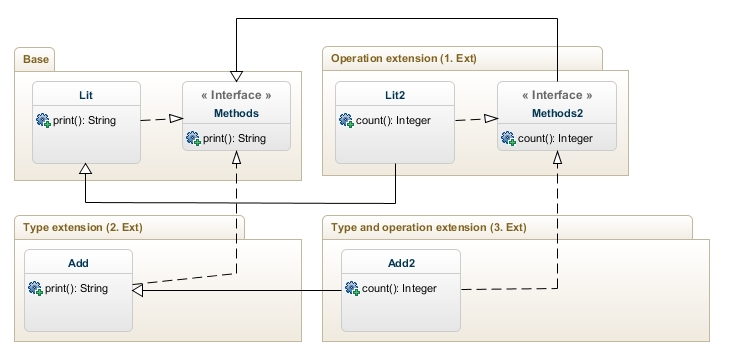
\includegraphics[width=330px,keepaspectratio=true]{Expression_problem-diag.jpg}

\caption{Class diagram of the example}
\label{exampleClassDiagram}
\end{figure}

The third extension will give us an Error because the fields "left" and "right" are of the type "Methods" and do not have a Method "count".

\section{Suggested solution}
\label{suggestedEPSolution}
\subsection{Return Collection Objects Instead Of Results}

The object algebra Oliveira et al \cite{Oliv-Extensibility-2012} used are returning not plain atomic values (like "string" for the print-method) but operation-specific objects \ref{iPrint} on which the operation can be called. To add the support of methods depending on other methods, we just need to combine the depending operations into the interface. We can take the interface Methods2 in Figure \ref{exampleFirstExtension}.

\begin{figure}[h]
\begin{lstlisting}[language=java]
    interface IPrint {
        String print();
    }
\end{lstlisting}
\caption{Extensibility for the masses \cite{Oliv-Extensibility-2012} page 8}
\label{iPrint}
\end{figure}

Count is not depending on print, but if we wanted to add an operation like "countPrintSpace", that would count the characters a print-method would return and therefore is depending on the print-method, another object algebra would have to duplicate the code of the first. So an object algebra that would return an object that implements Methods2 could have also implement depending methods.

\subsection{Multi Purpose Object Algebra Interface}

To generate such aggregated objects we need an object algebra, that factorizes those. Every type has an algebraic signature \cite{Oliv-Extensibility-2012} that the algebra has to match. This is also the location where we would add new types. For the reference to other abstract expressions we use the type-params (symbol "A") also in the parameters of the type-constructors (Example in figure \ref{algebraInterfaces}). Every algebra implementing these interfaces has to set a type param (like "Methods2" in figure \ref{exampleFirstExtension}) that injects the family-dependency to the entity.

\begin{figure}[t]
\begin{lstlisting}[language=java]
    public interface Types <A> {
        public A lit(Integer x);
    }
    public interface Types2 <A> extends Types <A> {
        public A add(A e1,A e2);
    }
\end{lstlisting}
\caption{Interfaces for algebras with the signature of the types}
\label{algebraInterfaces}
\end{figure}

\subsection{Factorizing The Object}

As in the example of the anonymous class implementing the IPrint-Interface, we return a Methods2-object, that implements the operations we want to add. This anonymous class could also be seen as the implementation of the generic "Lit"- and "Add"-classes. For operations that are derived from a super-type, we would have to extend the classes. We want to support multiple inheritance to meet the requirement for independent extensibility so instead we delegate the calls (see section "Multiple Inheritance" \ref{multipleInheritance}).

\begin{figure}[b]
\begin{lstlisting}[language=java]
public class Algebra4 implements Types <Methods2> {
    public Methods2 add(final Methods e1, final Methods e2) { 
      final Methods _instance = new Algebra3().add(e1, e2);
      return new Methods2() {
               public Integer count() {
                   return e1.count() + 1 + e2.count();
               }
               public String print() {
                   return _instance.print();
               }
           };
    }
    public Methods lit(Integer x) { 
      final Methods2 _instance2 = new Algebra2().lit(x);
      final Methods _instance3 = new Algebra3().lit(x);
      return new Methods2() {
               public Integer count() { 
                   return _instance2.count();
               }
               public String print() { 
                   return _instance3.print();
               }
           };
    }
\end{lstlisting}
\caption{The resulting Algebra-object for the third extension (Algebra2 and Algebra3 likewise)}
\label{algebraInterfaces}
\end{figure}

Notice that in the Lit.print()-implementation we could either use \_instance2 or \_instance3 to delegate. Coincidentally both will refer to the same operation. To find the best ancestor to refer to one would use a linearization like suggested from Bracha \cite{Bracha-Mixin-1990}.

\subsection{Features}

With this use of object algebras we have some benefits over the the suggested solution by Oliveira et al with the trade off of boilerplate code which we will overcome in the chapter "Desugaring with SugarJ" \ref{sugarJChapter}. Many requirements were met yet:

\begin{itemize}
\item Statefulness: We can save the state in fields to the anonymous classes that can be used in the methods like in any other class.

\item Serialization: The anonymous classes are just some syntactical sugar that Java translates into native Java-classes, so any kind of serialization will work just fine.

\item Intern method calls: The delegation is encapsulated into the methods so the cross-calls from one to another method in the same class works.
\end{itemize}

Not met yet:

\begin{itemize}
\item Ease of use: Because of the boilerplate code, the manual use of this solution is not as simple as the generic types. The use of the objects in other contexts however works like with the generic types.
\end{itemize}

\subsection{Differences to Oliveira et al \cite{Oliv-Extensibility-2012}}

The decoupling of explicit method binding to one interface is one of the great strength in the solution of Olivera et al, but in some cases it is not needed or even it is important to call dependent methods. Although their work does not explicit limit this, our extension tries to overcome the independent extension with delegation to ancestors to also support multiple inheritance. With this comes a trade off to have much delegation boiler code.

The "step back" to classes, that have many combined methods with state fields is meant to lower the challenge to this solution.  

Instead of an object algebra for every new method, the combined object algebras follow a derived interface, that grows with the new methods.

\subsection{Multiple Inheritance}
\label{multipleInheritance}

Java does not support multiple inheritance genuinely, but we need it to support independent extensions, we have to use a special delegation to refer to super methods in multiple super classes. Not implemented methods that need to be derived from a super-type have to be delegated to a static object that is instantiated with the construction of the entity-object. The solution to multiple inheritance with delegation is derived from \cite{Tempero-Multiple-2000} and modified to use final variables in the factory instead of instantiating the super objects in the constructor of the class.

\subsection{Visibility}
\label{expressionProblemVisibility}

With delegation instead of inheritance, the full visibility features of Java cannot be supported. There is no easy way to cover the protected visibility with delegation. Instead we will consider it as being not possible. Public methods can easy be delegated to the static objects and private fields and methods do not need delegation (because they can only be called in the defining class context).

Public field access cannot be delegated because Java does not have features to catch such calls. Instead we consider the need for getter and setter methods.

\subsection{Combining The Parts}
\label{combiningTheParts}
The naming of the interfaces and algebras would be very confusing if they would just be enumerated. Therefor we suggest a form to define the interfaces and classes in a combined class (see figure \ref{combinedClass}).

\begin{figure}[t]
\begin{lstlisting}[language=java]
public class [Familyname] {
  public interface Types<A> {
    public A [TypeName]([TypeParams]);
    [...Types...]
  }
  public interface Methods { 
    public [MethodReturnType] [MethodName]([MethodParams]);
    [...Methods...]
  }
  public class Algebra implements Types<Methods> { 
    public Methods [TypeName](final [TypeParams]) {
      return new Methods() {
           public [MethodReturnType] [MethodName]([MethodParams]) { 
             [...]
           }
           [...Methods...]
      };
    }
    [...Types...]
  }
  protected static Algebra _algebra;
  public static Algebra Algebra()
  { 
    if(_algebra == null)
      _algebra = new [FamilyName]().new Algebra();
    return _algebra;
  }
}
\end{lstlisting}
\caption{Combining algebra interface (\emph{Types}), resulting family interface (\emph{Methods}), algebra (\emph{Algebra}) and Singleton for the algebra}
\label{combinedClass}
\end{figure}

To address an object of this family, one would reference [Familyname].Methods. The singleton method "algebra()" is for convenience and memory usage reasons.

\chapter{Syntax Extension For The Solution}
\label{syntaxExtensionEP}
The solution has too much boilerplate code to use it efficiently. To come over this, we create a syntax that consists of only the variable parts.

\section{Family}

Expression elements have the same interface. A Family is a way to couple the entities to be part of the expression. In this family, every class implements the family interface. Every public operation that exists in one of the classes of the family has to be in every other of them. Families can extend each other independent. Every derived Family inherits the public methods of the super families and has to implement the missing methods to the classes. Methods in families can be overwritten.

An interface family of the third extension of our example, where IntSub and IntCount are the first and second extending families would only implement the missing method "count" on the entity "Add" (See figure \ref{thirdExtensionFamily}).

\begin{figure}[h]
\begin{lstlisting}[language=exprExt]
family IntAddCount extends IntAdd,IntCount {
    class Add (IntAddCount e1,IntAddCount e2) {
        public Integer count () {
            return new Integer(e1.count() + 1 + e2.count());
        }
    }
}
\end{lstlisting}
\caption{The third extension as family}
\label{thirdExtensionFamily}
\end{figure}

As convention to reference to a family dependent type we will use the family name as type.

\section{Strip Boilerplate Code}

The delegation code can mostly be generated. To do this, we only need the information about the super-families. This information includes which families and in which order it inherits from them. Also the anonymous classes, the interfaces and the object algebra interface can be generated. The goal is to keep the new syntax as simple as possible and extensively as necessarily.

\section{Cognitive Dimensions}

\subsection{Consistency}

The consistency of a language describes if someone who learnt part of a language, could easily adapt other features of the language. For syntax extensions that extend a complete language with syntactical sugar it is very important to keep that in mind in their implementation. The main goal of syntax extensions is to simplify features, that would otherwise be difficult to implement.

The Interface family meets this requirement, because it consists of classes, that have mostly the same syntax and features as every other class a user would write. The context of an interface family has the same symbols as an interface would have. The binding of the classes in the family to the interface name communicates the outer interface to be met by the inner classes.

Because multiple inheritance is not part of Java, a given algorithm to delegate derived calls to the super objects is not forced. So the reversed extend-order does not violate this rule.

\subsection{Viscosity}

The viscosity of a language describes the effort that is required to perform a single change. As long as it does not conflict with the readability of the code, the lower the effort, the better is this condition met.

In the interface family syntax, the effort for a change is very low. Because every method that is added to a class will extend the interface and every type that is defined in the interface family will implement the interface the interface does not have to be updated explicitly. To extend a class, you simply have to define it, without the need to know if it was already derived from a previous interface family and if, which methods.

\subsection{Progressive Evaluation}

Progressive evaluation describes if a developer gets feedback in a partially-complete program.

Our draft does not support this now, because of the need of static type checks, but it would be possible in a future implementation to allow methods that have not been implemented in a type could throw an exception but the compiler would now fail on a missing method.

\section{Limitations}

Although the syntax extension alone is only limited by the ideas we have, we will provide a solution to desugar this syntax to valid Java code that is based on our solution to the expression problem (See Section "Suggested Solution" \ref{suggestedEPSolution}). There are a few limitations that the desugaring brought with us. To some of the limitations we will provide a potential solution that we could not prove, to a few we only had an idea.

\subsection{Visibility}

This was already discovered in chapter "The Expression Problem" \ref{expressionProblemVisibility} and has its reason in the delegation instead of inheritance.
The class knows only public methods, private methods and private fields.

\subsection{Multiple Inheritance Linearization}

The inheritance order follows a simple hierarchical order. Calls to derived methods are delegated to the first Family Interface that has the method in reversed order of the "extends" keyword. Although a linearization like with \emph{Mixins} suggested by Bracha \cite{Bracha-Mixin-1990} would have been more straight-forwarded, the implementation of this algorithm would have been too difficult to implement to include it into this work.

% Hier eine Referenz zu einer potenziellen Lösung im nächsten Kapitel

\subsection{Inheritance within family members}

Subtyping of family members from other family members or from outer the family is not genuinely supported. One could implement a delegation to a depending class.

\subsection{Instantiation of Members from the Inner Code}

Although you can instantiate new members of the same family with using the \_algebra field, the dependencies of a derived family are not met because there is no method to get to the caller family \_algebra-field.

\chapter{Desugaring With SugarJ}
\label{sugarJChapter}

\section{SugarJ}
We want to use SugarJ \cite{Erdweg-SugarJ-2011} to inject the defined syntax extension to an IDE that supports such syntax extensions. As SugarJ uses Spoofax, a framework to dynamically load new syntax definitions into IDEs to work with new (derived) languages \cite{Kats-Spoofax-2010}.

\subsection{SDF}
SugarJ uses SDF \cite{Heering-SDF-1989, Brand-SDF-2007} a formalism to define syntax. There is already a SDF of Java language available in the SugarJ repository \cite{Java-SDF-2014} where one can lookup design and structure of the language and find information about how to derive his own language extensions. With this definition an IDE, that supports the Spoofax framework like eclipse is able to parse, verify and syntax highlight code, that is written in this new syntax.

\subsection{Stratego/XT}
% Check of das stimmt:
In the second step, SugarJ uses Stratego/XT (\cite{Stratego-Manual, Kats-Spoofax-2010}) to take the aterm (tree representation of a whole syntax representation in SDF) of a language and transform it with various rules to remove every non-terminal that might be added by the previous SDF by rewriting parts of the aterm.

\subsection{Desugaring}
These two technologies in combination with the Spoofax framework can be used to define new domain languages (SDF), that an IDE can use to utilize (Spoofax), and afterwards transform into valid code in an existing language (Stratego). This process is called \emph{Desugaring}, because syntactical sugar that one would match with a language extension via SDF is transformed in the generic code in another language, that assigns the idea of the domain language into it.

\section{Experience with SugarJ}
In this section we will describe our subjective view on the development-process with SugarJ.

\subsection{Installation and IDE}
The installation is pretty straight-forwarded and through the eclipse software installation dialog very easy. The instructions can be found on the official site of SugarJ \cite{SugarJ-Homepage}. The interpreter has to be aligned in the target project and a suggestion to push the Java environment variables, but that is all, that is needed to do by hand. When opening a .sugj-file you have a few options to start: Import an existing "Sugar", define your own "Sugar" or use syntax that goes through the process as described (SDF matching, Stratego rewriting). The transform menu gives an easy way to generate aterms from existing code to get a feeling for aterm-transformation of existing code in Java as well as existing SugarJ-code.

\section{Families in SugarJ}

In this section we will describe how we used SugarJ to define our syntax extension in \ref{syntaxExtensionEP} and transform it to the solution we presented in \ref{suggestedEPSolution}.

\subsection{Defining the Syntax Extension}
The syntax definition is the comparable easy part of the desugaring. We needed a point to step into the java language. We chose the \emph{JavaTypeDec} as it is the top level\footnote{On top of that are only imports and namespaces which cannot be matched by SugarJ, because they are used to define which SugarJ-library will be used.} of declaration in Java, where every class, interface, etc. is declared. We defined a new keyword "family" and brought it into context with our own structure. To not reinvent the wheel, we referred to the generic Java non-terminals as often as possible (i.e. JavaClassBody, we do not have to redefine what a class-body contains of). After that, the new syntax could be matched.

\subsection{Rewriting the Syntax Extension to Java-Code}


\chapter{Other Work In This Domain}


\chapter{Use Case}

As proof, that in a working environment this work saves much manual writing and decouples the functional extensions and the type extensions, here is a real life example:

\begin{lstlisting}[language=exprExt]
family ShapeSquare {
    class Square (Float x) {
        public Float area () {
            return x*x;
        }
    }
}
family ShapeSCircleTriangle extends Shape {
    class Circle (Float r) {
        public Float area () {
            return Math.PI * r * r;
        }
    }
    class EquilateralTriangle (Float a) {
        public Float area () {
            return Math.sqrt(3)/4 * a * a;
        }
    }
}
family ShapeSCTCircumLength extends ShapeSCircleTriangle {
    class Square (Float x) {
        public Float circumferenceLength() {
            return 4 * x;
        }
    }
    class Circle (Float r) {
        public Float circumferenceLength() {
            return 2 * Math.Pi * r;
        }
    }
    class EquilateralTriangle (Float a) {
        public Float circumferenceLength() {
            return 3 * x;
        }
    }
}
family ShapeSCTTupleShapeCircumLength
        extends ShapeSCTCircumLength {
    class TupleShape (ShapeSCTTupleShapeCircumLength first,
                      ShapeSCTTupleShapeCircumLength second) {
        public Float area () {
            return first.area() + second.area();
        }
        public Float circumferenceLength() {
            return first.circumferenceLength()
                + second.circumferenceLength();
        }
    }
}
family ShapeSCTEllipse extends ShapeSCircleTriangle {
    class Ellipse (Float r1, Float r2) {
        public Float area() {
            return Math.PI * r1 * r2;
        }
    }
}
family ShapeSCTECircumLength
        extends ShapeSCTEllipse, ShapeSCTCircumLength {
    class Ellipse (Float r1, Float r2) {
        public Float circumferenceLength() {
            return Math.PI * ( 3 * ( r1 + r2 ) - Math.sqrt(
                    10 * r1 * r2 + 3 * ( r1 * r1 + r2 * r2 )
                ) ); // Ramanujan approximation
        }
    }
}
family ShapeSCTECTSACRatio extends ShapeSCircleTriangle {
    class TupleShape (ShapeSCTECTSACRatio first,
                      ShapeSCTECTSACRatio second) {
        public Float areaCircumferenceRatio() {
            return area()/circumferenceLength();
        }
    }
    class Ellipse (Float r1, Float r2) {
        public Float areaCircumferenceRatio() {
            return area()/circumferenceLength();
        }
    }
    class Square (Float x) {
        public Float areaCircumferenceRatio() {
            return x/4;
        }
    }
    class Circle (Float r) {
        public Float areaCircumferenceRatio() {
            return r/2;
        }
    }
    class EquilateralTriangle (Float a) {
        public Float areaCircumferenceRatio() {
            return Math.Sqrt(3)/12 * a;
        }
    }
}

\end{lstlisting}

\bibliographystyle{plain}

\bibliography{testFile} % no suffix

\end{document}

















